\documentclass[12pt]{book}
\usepackage[utf8]{inputenc}
\usepackage[T1]{fontenc}
\usepackage{tocbibind}
\usepackage{mathptmx}
\usepackage{geometry}
\usepackage{mathtools}
\usepackage[english]{babel}
\usepackage{graphicx}
\usepackage{subcaption}
\usepackage{stackengine}
\usepackage[os=win]{menukeys}
\usepackage{hyperref}
\usepackage{xcolor}
\usepackage{color}
\usepackage{tikz}
\usepackage[yyyymmdd,hhmmss]{datetime}
\usepackage{etoolbox}
\usepackage[inline]{enumitem}
\usepackage{listings}
\usepackage{booktabs}
\usepackage[os=win]{menukeys}
\usepackage{minted}

\newcommand{\WindowsLogo}{\raisebox{-0.1em}{
\includegraphics[height=0.8em]{images/logo/Windows_3_logo_simplified}}}
%\newcommand{\PowerLogo}{\raisebox{-0.1em}{\includegraphics[height=0.8em]{images/logo/power}}}
\newcommand{\WinKey}{\keys{\WindowsLogo}}
\newcommand{\PowerKey}{\keys{\PowerLogo}}

%%%%% Mengganti label "Contents" ke "Daftar Isi" %%%%%
\addto\captionsenglish{\renewcommand{\contentsname}{Daftar Isi}}

%%%%% Mengganti label "Chapter" ke "Bab" %%%%%
\addto\captionsenglish{\renewcommand{\chaptername}{Bab}}

%%%%% Mengganti label "Figure" ke "Gambar" %%%%%
\addto\captionsenglish{\renewcommand{\figurename}{Gambar}}

%%%%% Mengganti label "List of Figures" ke "Daftar Gambar" %%%%%
\addto\captionsenglish{\renewcommand{\listfigurename}{Daftar Gambar}}

%%%%% Mengganti label "Table" ke "Tabel" %%%%%
\addto\captionsenglish{\renewcommand{\tablename}{Tabel}}

%%%%% Mengganti label "List of Tables" ke "Daftar Table" %%%%%
\addto\captionsenglish{\renewcommand{\listtablename}{Daftar Tabel}}

\hypersetup{
	colorlinks=true, %set true if you want colored links
	linktoc=all,     %set to all if you want both sections and subsections linked
	linkcolor=blue,  %choose some color if you want links to stand out
	urlcolor=blue,   %url color
}

\geometry{
	a4paper,
	left=10mm,
	right=10mm,
	top=15mm,
	bottom=15mm,
}

\date{}

\hypersetup{citecolor=black}

\definecolor{LightGray}{gray}{0.95}

%\pagecolor[rgb]{0.1,0.1,0.1}
%\color[rgb]{1,1,1}

\lstset
{
	language=bash,
	breaklines=true,
	basicstyle=\tt\normalsize,
	frame = single
}

\begin{document}
    \frontmatter
	\begin{titlepage}
		\centering
		{\LARGE \bf Usulan Pengukuran Prototype Audiometri Portable}
		\vfill
		{\Large Achmadi ST MT}
		\vfill
		Update: {\today}
		\vfill
		
\includegraphics[width=250pt]{images/logo/logoviblab}
		\vfill
		\vfill
		\vfill
	\end{titlepage}

	%%%%%%%%%%%%%%%%%%%%%%%%%%%%%%%%%%%%%%%%%%%%%%%%%%%%%%%%%%%%%%%%%

	\newpage
	\tableofcontents
	\listoffigures
	\listoftables

	%%%%%%%%%%%%%%%%%%%%%%%%%%%%%%%%%%%%%%%%%%%%%%%%%%%%%%%%%%%%%%%%%

    \mainmatter
    \newpage

	\chapter{Persiapan}

    Berikut Penjelasan singkat terkait persiapan paket purwarupa

	\section{Hardware}

    Berikut adalah perangkat keras yang perlu disiapkan untuk pengujian ini meliputi:

    \begin{enumerate}
		\item Unit Prototype Konsol Audiometri yang akan diuji.
		\begin{figure}[!ht]
			\centering
			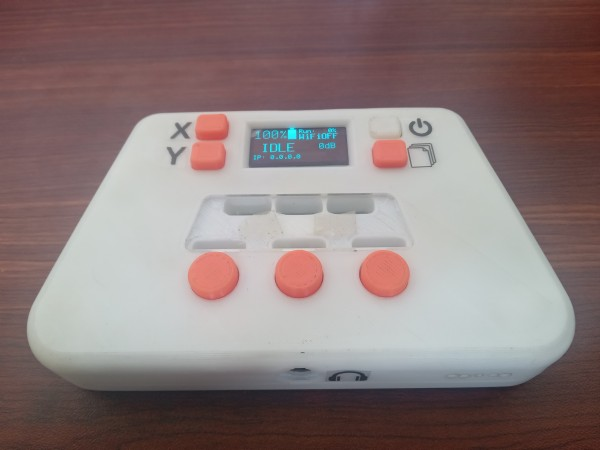
\includegraphics[width=250pt]{images/unit/proto}
			\caption{Unit Prototype}
		\end{figure}

		\item Kabel Micro-USB ke USB-A.
		\begin{figure}[!ht]
			\centering
			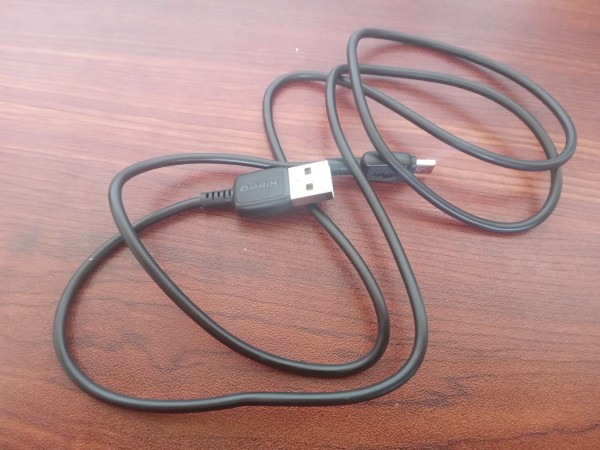
\includegraphics[width=200pt]{images/unit/kabel}
			\caption{Kabel USB}
		\end{figure}

		\newpage
		\item Wired-Headphone yang telah terpaket
		\begin{figure}[!ht]
			\centering
			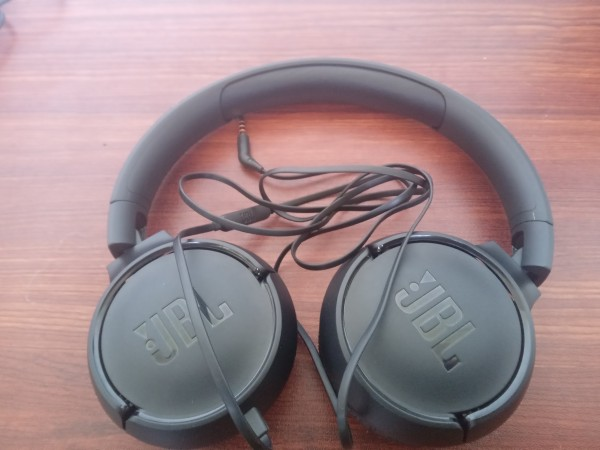
\includegraphics[width=200pt]{images/unit/jbl}
			\caption{Wired Headphone}
		\end{figure}

        \item MiniDSP EARS
         \begin{figure}[!ht]
			\centering
			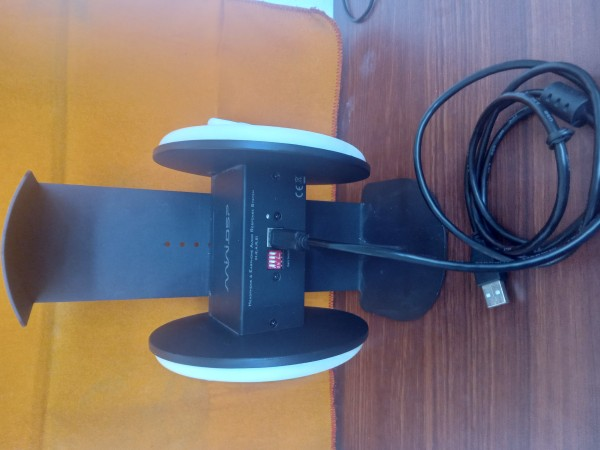
\includegraphics[width=200pt,angle=-90]{images/unit/ears}
			\caption{MiniDSP EARS}
		\end{figure}

     \end{enumerate}

    \section{Pemasangan}

	Berikut langkah pemasangan unit perangkat di atas:

	\begin{enumerate}
		\item Pasang Headphone pada unit EARS sebagaimana jika digunakan pada telinga manusia.
		Pastikan kiri dan kanan tidak terbalik.
		Pastikan Headphone menutup lubang telinga.

		\newpage
		\begin{figure}[!ht]
			\centering
			\begin{subfigure}[t]{0.35\textwidth}
				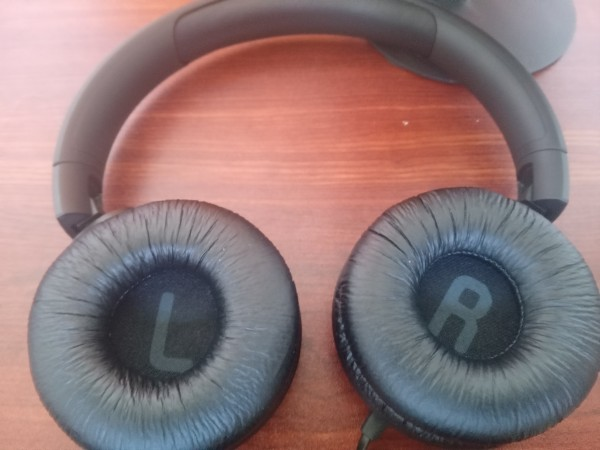
\includegraphics[width=\textwidth]{images/pasang/chjbl}
				\caption{Label Channel}
			\end{subfigure}
			\begin{subfigure}[t]{0.35\textwidth}
				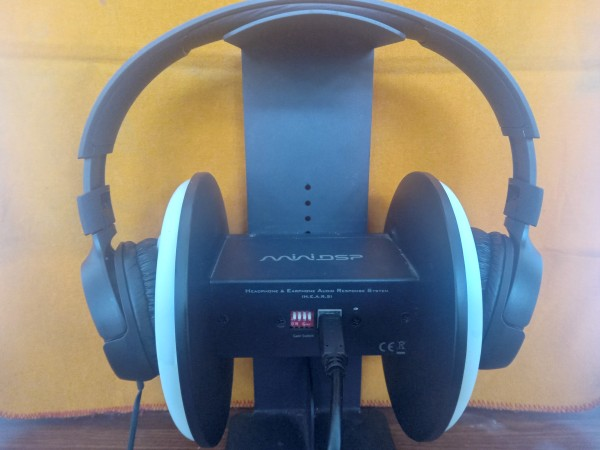
\includegraphics[width=\textwidth]{images/pasang/pasangjbl}
				\caption{Pasang Headphone}
			\end{subfigure}
			\\
			\begin{subfigure}[t]{0.35\textwidth}
				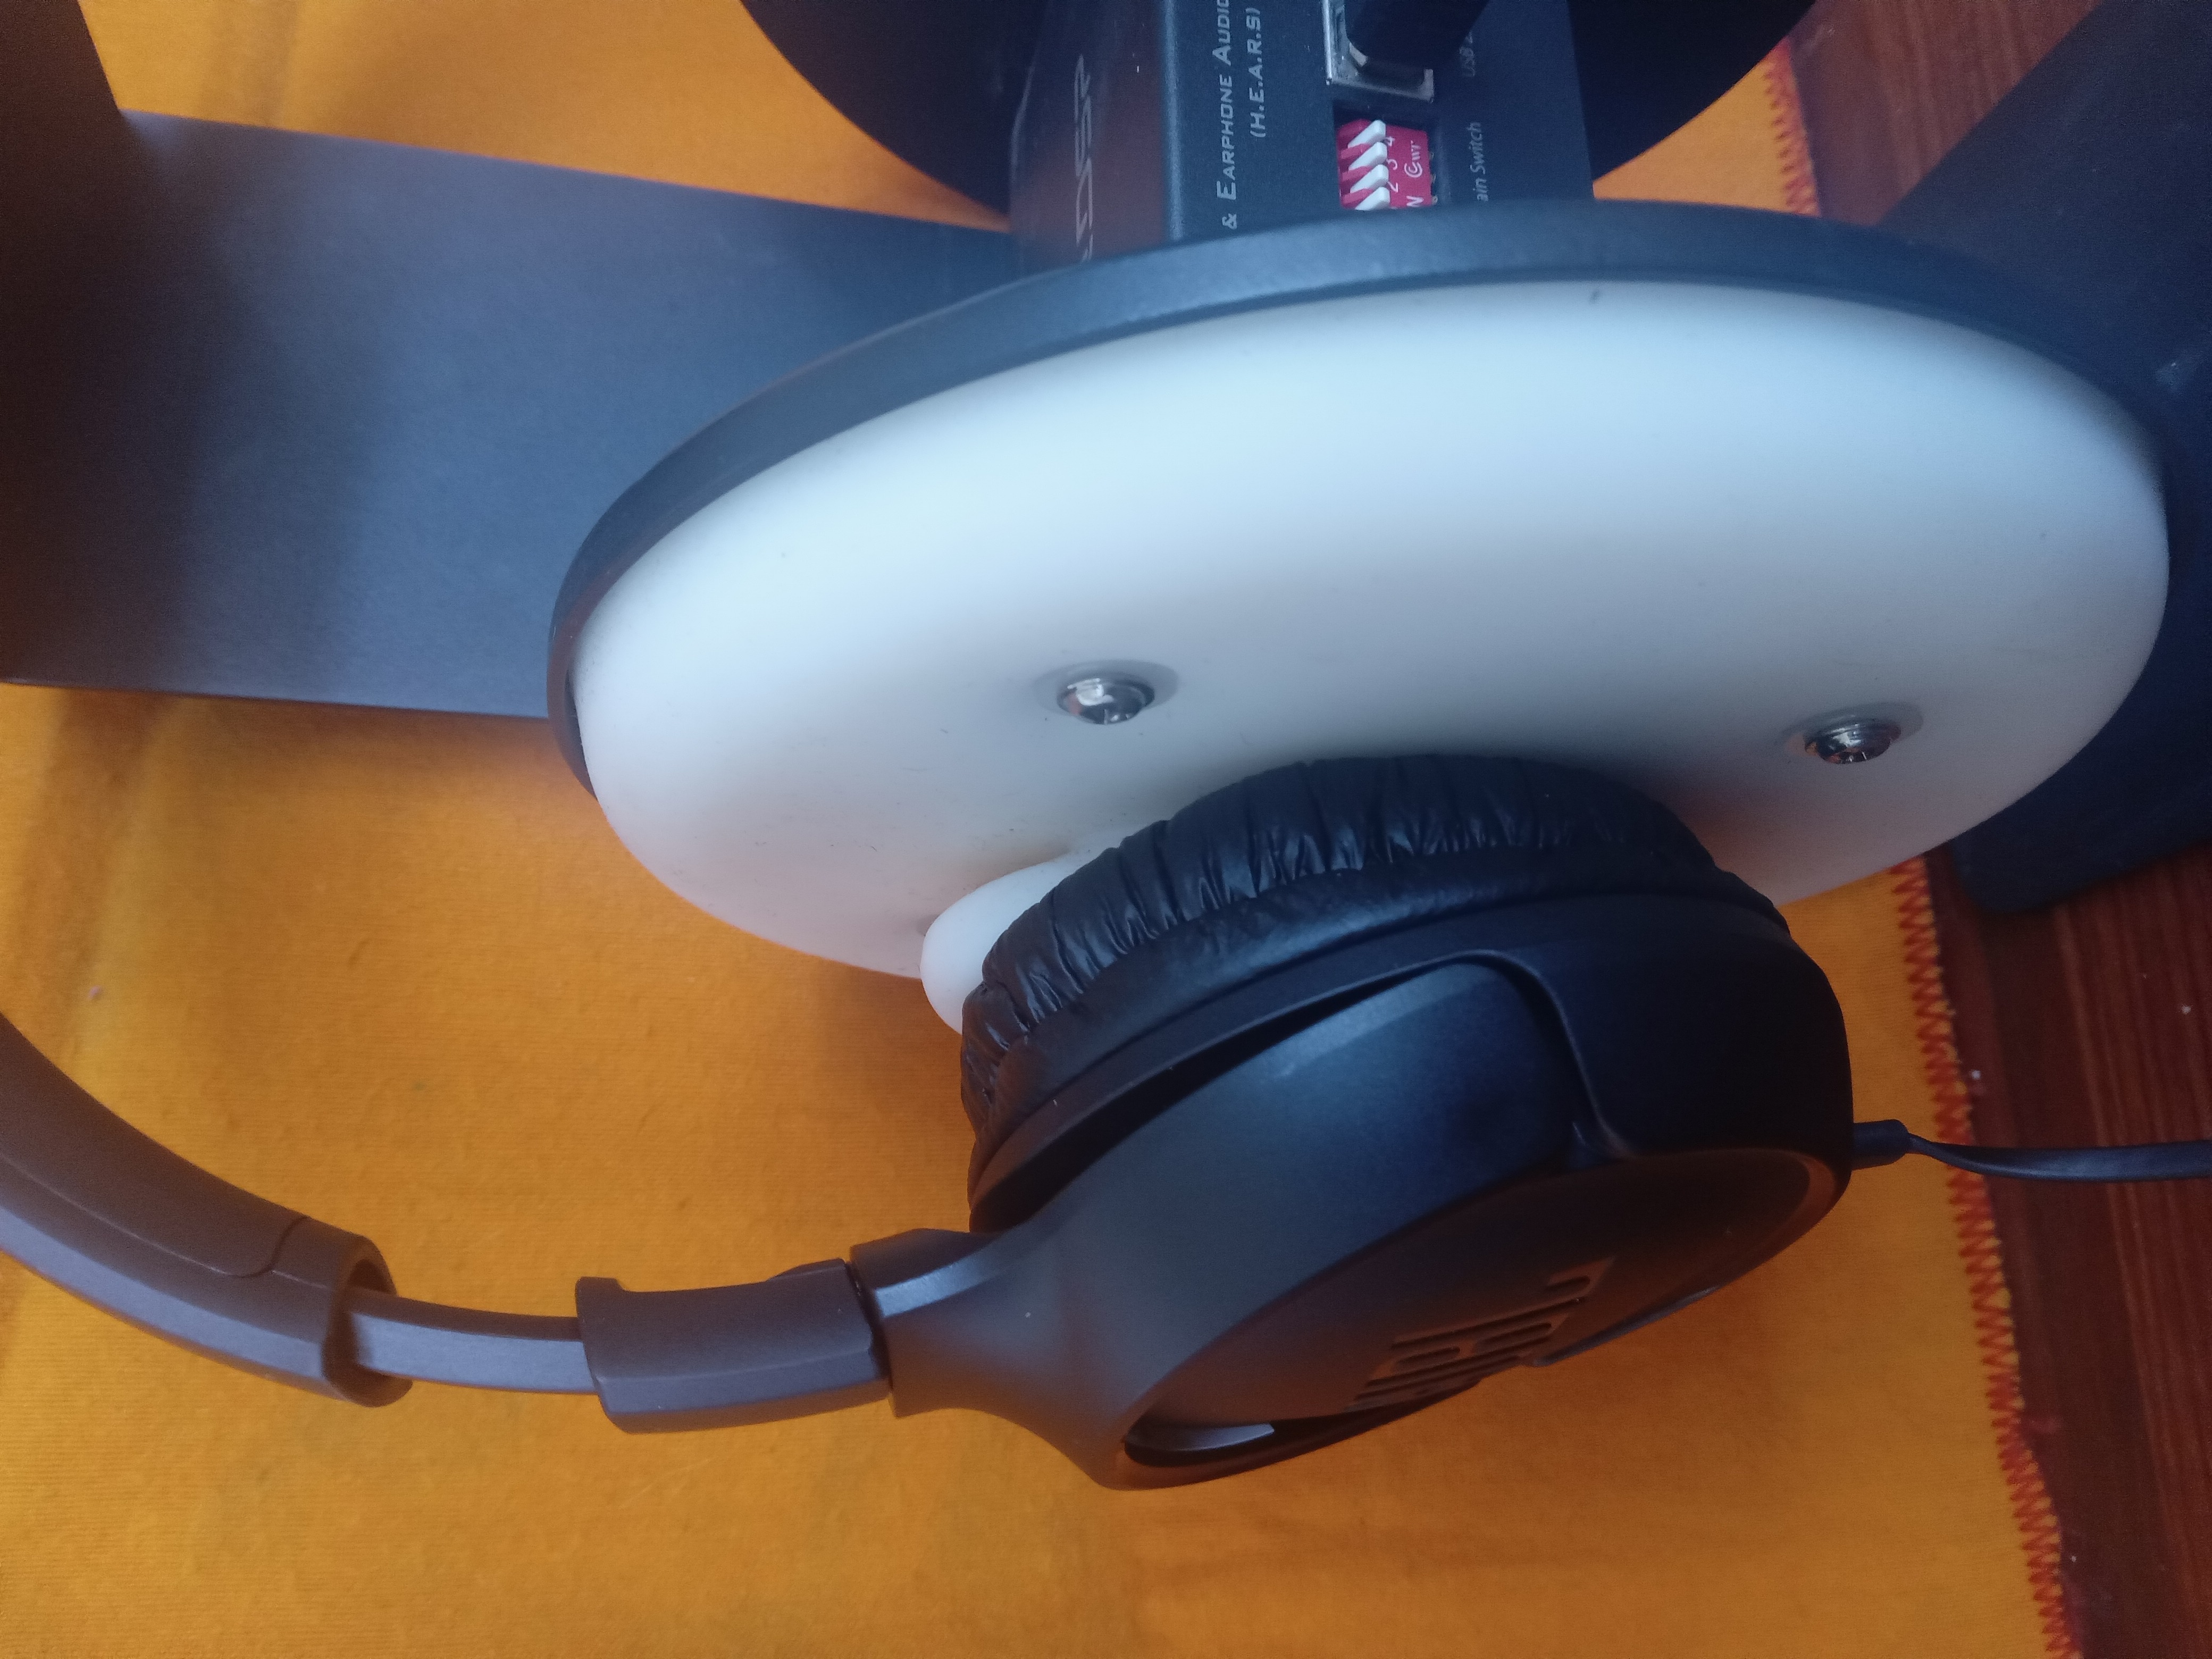
\includegraphics[width=\textwidth,angle=-90]{images/pasang/tutupjbl}
				\caption{Menutup Telinga}
			\end{subfigure}

			\caption{Pemasangan Headphone pada EARS}
		\end{figure}

		\item Sambung Jack Audio Headphone ke Konsol
		\begin{figure}[!ht]
			\centering
			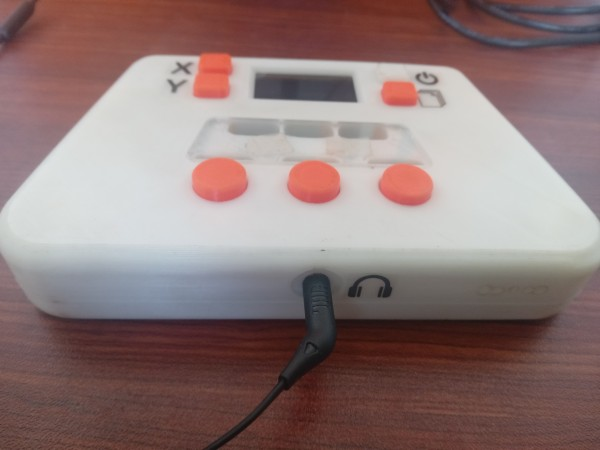
\includegraphics[width=200pt]{images/pasang/sambung_audio}
			\caption{Sambung Jack Audio}
		\end{figure}

		\newpage
		\item Nyalakan Unit. Tunggu hingga LED biru berkedip.
		\begin{figure}[!ht]
			\centering
			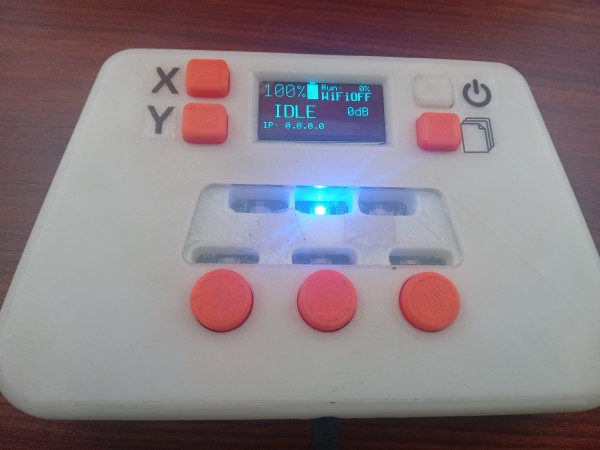
\includegraphics[width=200pt]{images/pasang/nyalakan_unit}
			\caption{Nyalakan Unit}
		\end{figure}
		\item Sambung Kabel USB ke Konsol
		\begin{figure}[!ht]
			\centering
			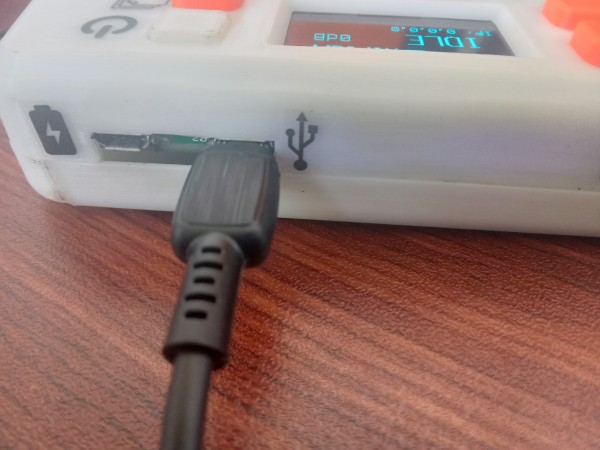
\includegraphics[width=200pt]{images/pasang/sambung_usb}
			\caption{Sambung Kabel USB}
		\end{figure}
	\end{enumerate}

    \section{Komunikasi Serial}

    Berikut adalah perangkat lunak komunikasi serial ke Konsol yang perlu disiapkan untuk pengujian ini
    (panduan ini menggunakan Windows-7 32-bit sebagai contoh):

    \begin{enumerate}
    	\item Install driver ARM USB-CDC.\\
    	Untuk dapat menghubungkan unit prototype dengan komputer,
    	diperlukan driver ARM USB-CDC untuk komunikasi serial.

    	\begin{itemize}
    		\item File installer (sesuaikan dengan bit OS).
    		Dapat didownload di \href{https://drive.google.com/drive/folders/19gXVrxR68SFHQUGGGgKb0Da03oV7Rh41?usp=share_link}{USB-CDC\_Driver}.
    		\begin{figure}[!ht]
    			\centering
    			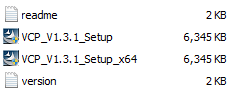
\includegraphics[width=200pt]{images/software/driver}
    			\caption{Installer Driver}
    		\end{figure}

    		\newpage
    		\item Instalasi driver (tanpa unit prototype terhubung) cukup mudah sebagaimana umumnya.
    		\begin{figure}[!ht]
    			\centering
    			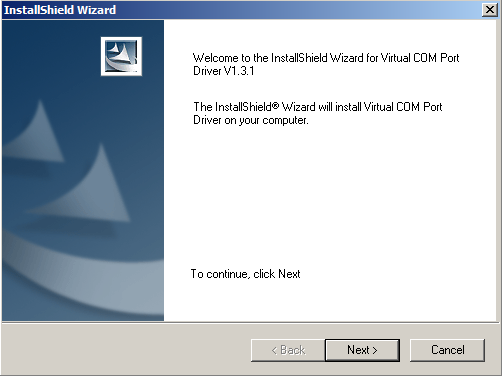
\includegraphics[width=200pt]{images/software/install_driver}
    			\caption{Mulai instal driver}
    		\end{figure}
    	\end{itemize}

    	\item Sambungkan unit prototype yang telah nyala dengan komputer via kabel USB.
    	\begin{figure}[!ht]
    		\centering
    		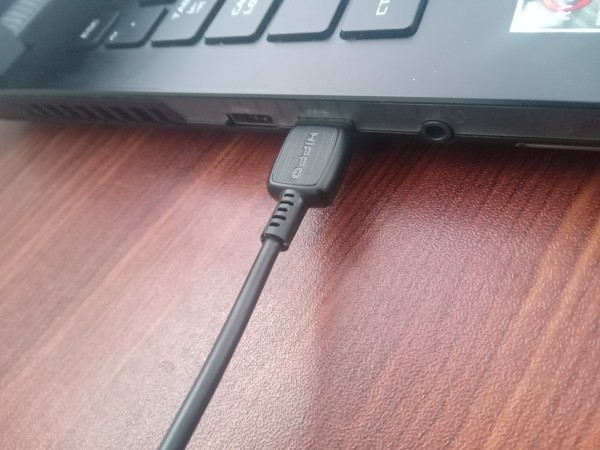
\includegraphics[width=200pt]{images/pasang/laptop_usb}
    		\caption{Sambung Kabel USB ke Laptop}
    	\end{figure}

    	\item Tunggu hingga driver selesai mengkonfigurasi otomatis

    	\item Cek \textit{Device Manager} untuk mengetahui Nomor Serial-Port
    	\begin{itemize}
    		\item Buka run-command dialog dengan kombinasi keyboard (\keys{\WinKey + r})

    		\item masukkan perintah \textbf{devmgmt.msc}.
    		\begin{figure}[!ht]
    			\centering
    			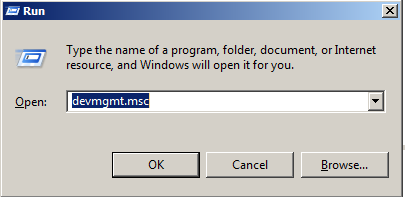
\includegraphics[width=200pt]{images/software/devicemgr}
    			\caption{Memanggil Device Manager}
    		\end{figure}

    		\item Tekan (\keys{\return}) atau klik OK

    		\newpage
    		\item Cari entry \textit{Ports (COM and LPT)}.
    		Catat nomor port untuk entry \textit{STMicroelectronics Virtual COM Port}.
    		Dalam contoh ini, terkonfigurasi pada COM3.

    		\begin{figure}[!ht]
    			\centering
    			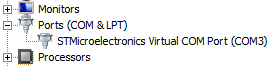
\includegraphics[width=200pt]{images/software/comport}
    			\caption{Serial Komunikasi pada COM3}
    		\end{figure}
    	\end{itemize}


    	\item Install Serial Terminal.
    	Untuk dapat berkomunikasi via serial port, perlu diinstall serial terminal.
    	Disini dicontohkan menggunakan \textit{Hercules}.

    	\begin{itemize}
    		\item Program terminal Hercules. Dapat didownload di \href{https://drive.google.com/drive/folders/1fgNPnGeSm20TrFfwmeCa4B24WIN_t_o_?usp=share_link}{Terminal}.
    		\begin{figure}[!ht]
    			\centering
    			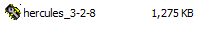
\includegraphics[width=200pt]{images/software/hercules}
    			\caption{Hercules Terminal}
    		\end{figure}

    		\item Jalankan program Hercules.
    		Jika muncul konfirmasi lisensi, cukup \textit{Close} saja.

    		\item Pilih tab \textit{Serial}.
    		\begin{figure}[!ht]
    			\centering
    			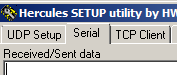
\includegraphics[width=200pt]{images/software/hercules_serial}
    			\caption{Serial Terminal}
    		\end{figure}
    	\end{itemize}

    	\item Test Komunikasi Serial
    	\begin{itemize}
    		\item Hercules Serial Terminal
    		\begin{figure}[!ht]
    			\centering
    			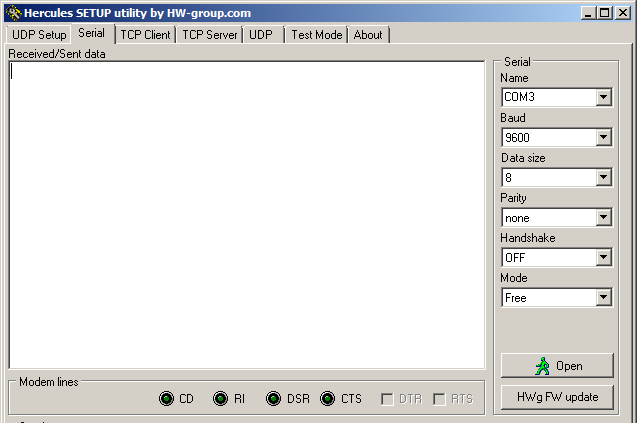
\includegraphics[width=250pt]{images/software/hercules_terminal}
    			\caption{Hercules Serial Terminal}
    		\end{figure}

    		\newpage
    		\item Setting Port pada Serial Terminal sebagai berikut
    		\begin{itemize}
    			\item Name     : COM3
    			\item Baud     : 9600
    			\item Data size: 8
    			\item Parity   : none
    		\end{itemize}

    		\begin{figure}[!ht]
    			\centering
    			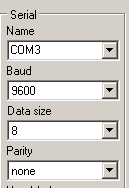
\includegraphics[width=100pt]{images/software/hercules_port}
    			\caption{Pengaturan serial port}
    		\end{figure}

    		\item Klik Open (pastikan unit prototype sudah standby dan terhubung
    		serta nama COM port sudah sesuai)

    		\begin{figure}[!ht]
    			\centering
    			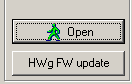
\includegraphics[width=100pt]{images/software/hercules_open}
    			\caption{Open Serial Port}
    		\end{figure}

    		\item Kolom terminal akan menampilkan pesan:
    		\begin{minted}[frame=lines,framesep=2mm,fontsize=\small]{text}
Serial port COM3 opened
    		\end{minted}

    		\item Selanjutnya, pada kolom terminal,
    		masukkan perintah berikut dan diakhiri dengan (\keys{\return})
    		\begin{minted}[frame=lines,framesep=2mm,fontsize=\small]{text}
info
    		\end{minted}
    		Serial akan menampilkan informasi kernel dan platform
    		\begin{figure}[!ht]
    			\centering
    			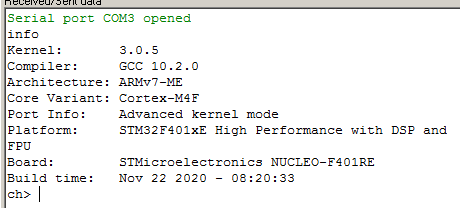
\includegraphics[width=300pt]{images/software/hercules_text}
    			\caption{Informasi Platform}
    		\end{figure}
    	\end{itemize}

    \end{enumerate}

	\newpage
	\subsection{Contoh Perintah Serial}

	Berikut beberapa contoh perintah serial yang dapat diakses melalui komunikasi serial Konsol:

	\begin{table}[!ht]
		\centering
		\begin{tabular}{|l|l|l|l|l|}
			\hline
			\textbf{No} & \textbf{Perintah} & \textbf{Fungsi} & \textbf{Contoh Perintah} & \textbf{Contoh Respon} \\
			\hline
			1 & \textit{coba} & Menguji Respon Serial & \textit{test} & \textit{Serial Console at 9600 \& buffer size 8 bit} \\
			\hline
			2 & \textit{help} & Menampilkan Perintah yang tersedia & \textit{help} & \textit{coba mmc out tes led sig tone virt ...} \\
			\hline
			3 & \textit{info} & Menampilkan Info Platform Chip & \textit{info} & \textit{Kernel: 6.1.4Compiler: GCC 12.1.0 ...} \\
			\hline
			4 & \textit{mmc} & Mengelola isi SDCard & \textit{mmc} & \textit{usage: mmc [test|ls|lsnum| ...} \\
			& & & \textit{mmc ls} & \textit{HT1.TXT HT2.TXT ...} \\
			& & & \textit{mmc cat 1} & \textit{\{"audiogram":\{ ...} \\
			\hline
			5 & \textit{out} & Menghasilkan nada murni &  \textit{out} & \textit{usage: out <0/1> <freq> <ampl> ...} \\
			& & & \textit{out 500 11} & \textit{Out: Freq:  500 Ampl:11} \\
			& & & \textit{out 1 250 8} & \textit{Out: Freq:  250 Ampl:8} \\
			\hline
		\end{tabular}
	\end{table}

	\textbf{Keterangan}: Beberapa keterangan perintah \textit{out}:
	\begin{itemize}
		\item Pilihan Channel adalah 0 atau kosong untuk kiri, dan 1 untuk kanan.
		\item Pilihan Frekuensi Nada Murni: 250Hz, 500Hz, 1000Hz, 2000Hz, 4000Hz, dan 8000Hz.
		\item Pilihan Skala Loudness Nada Murni: 1, 2, 3, 4, 5, 6, 7, 8, 9, 10, dan 11.
	\end{itemize}

	\newpage
    \section{Audio Analyzer}

    Untuk perangkat lunak Audio Analyzer, digunakan program \textit{Real-Time Analyzer}
    yang merupakan bagian dari paket software DSFF3 buatan Yoshimasha.
    Jika membutuhkan versi trial dapat didownload di \href{https://drive.google.com/drive/folders/1Z4cc4C_vb7BwU_MHDFyJTTVzQO7n7AHP?usp=share_link}{Audio\_Analyzer}.

    \begin{figure}[!ht]
    	\centering
    	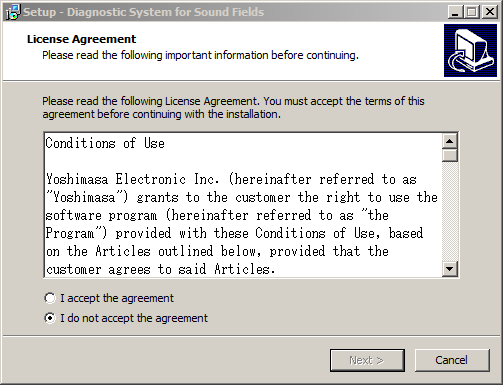
\includegraphics[width=300pt]{images/software/dssf3}
    	\caption{DSSF3}
    \end{figure}

    \subsection{Kalibrasi EARS}

    Proses kalibrasi dilakukan pada software Yoshimasa dengan pengatuan level 76 dBA/80dB (sesuai dengan kondisi perekaman suara di dalam ruang diffuse).
    Rekaman ruang diffuse dapat didownload di \href{https://drive.google.com/drive/folders/1FfFU9WPwoisH7j-oDqF8G0ruZmY0lxM_?usp=share_link}{EARS\_Calibration}\\

    \textbf{Catatan:} Tersedia pula rekaman untuk Tone 125Hz, namun direkomendasikan menggunakan rekaman derau untuk mencakup semua frekuensi.\\

    Berikut Langkah Kalibrasi:
    \begin{enumerate}
    	\item Jalankan program Realtime Analyzer, kemudian buka tab fungsi \textbf{FFT Analyzer} dan \textbf{Recorder}.
    	\begin{figure}[!ht]
    		\centering
    		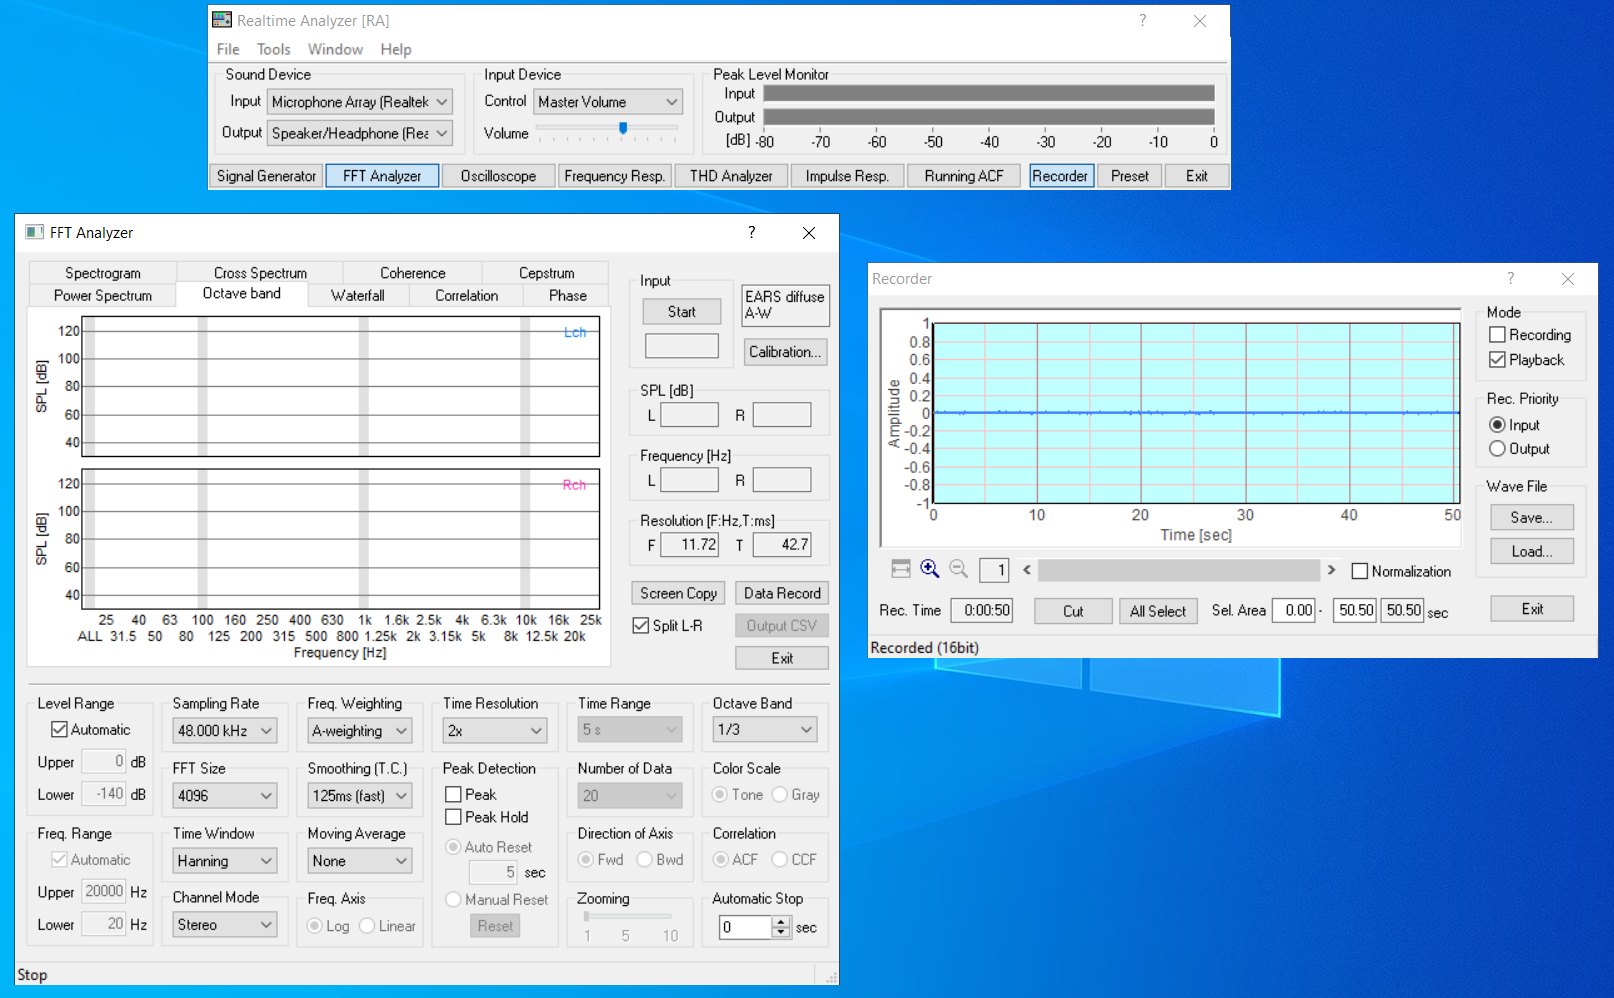
\includegraphics[width=0.6\textwidth]{images/kalibrasi/fft_analyzer}
    		\caption{FFT Analyzer}
    	\end{figure}

    	\newpage
    	\item Pada Jendela Recorder, klik \textbf{Load} untuk memasukkan rekaman
    	\begin{figure}[!ht]
    		\centering
    		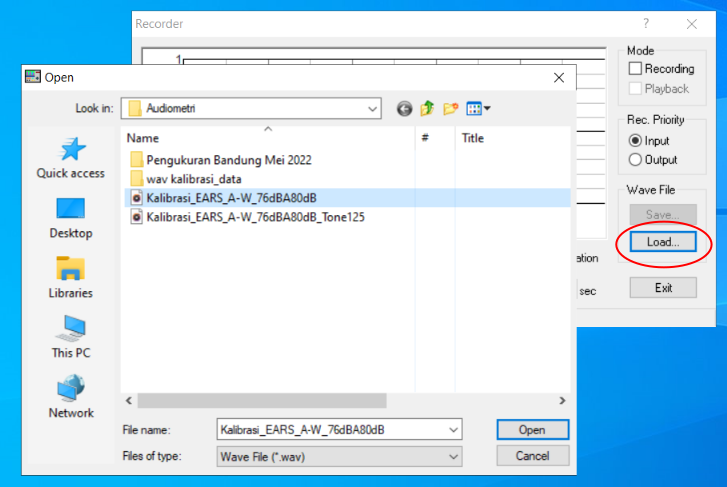
\includegraphics[width=0.65\textwidth]{images/kalibrasi/load_file}
    		\caption{Load File}
    	\end{figure}

    	\begin{figure}[!ht]
    		\centering
    		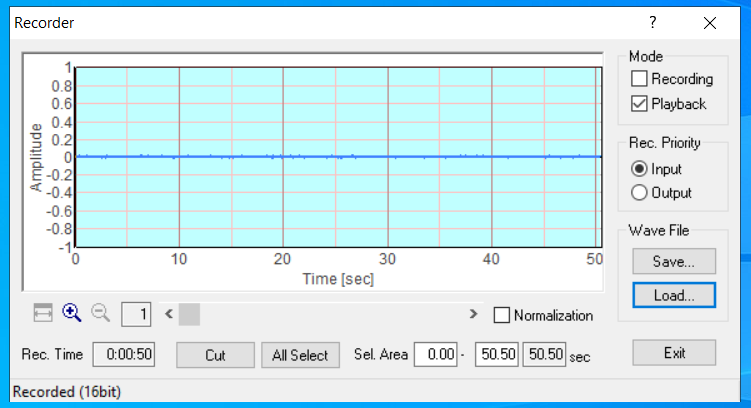
\includegraphics[width=0.65\textwidth]{images/kalibrasi/loaded}
    		\caption{Rekaman terload}
    	\end{figure}

    	\newpage
    	\item Pada Jendela FFT Analyzer, Klik \textbf{Calibration}.
    	Ikuti bagaimana panah dalam gambar di bawah dan atur nilai penyesuaian di 76dBA/80dB:

    	\begin{figure}[!ht]
    		\centering
    		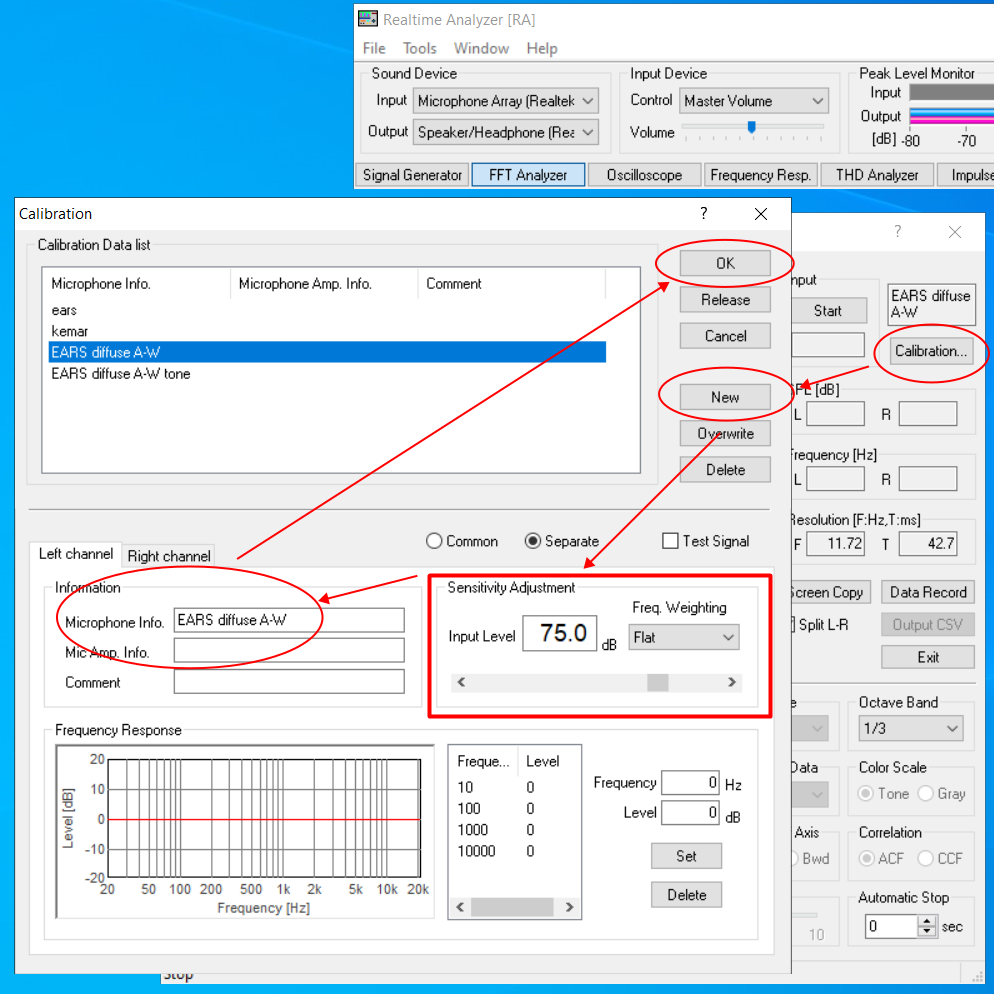
\includegraphics[width=\textwidth]{images/kalibrasi/adjustment}
    		\caption{Adjustment}
    	\end{figure}
    \end{enumerate}

	\newpage
	Antar-muka Real-Time Analyzer yang digunakan adalah \textit{FFT-Analyzer} pada tab \textit{Octave band}.

	\begin{figure}[!ht]
		\centering
		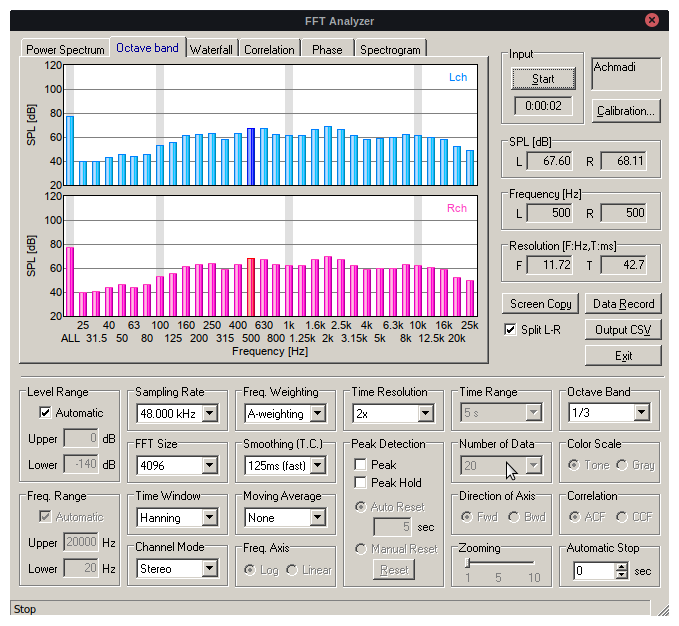
\includegraphics[width=\textwidth]{images/kalibrasi/fft}
		\caption{Octave band pada FFT analyzer}
	\end{figure}

    \chapter{Pengujian}

    \section{Test Tone-Generation}

    \section{Charging}

    \section{Rekomendasi Pengujian}
\end{document}

